% On two occasions I have been asked, – "Pray, Mr. Babbage, 
% if you put into the machine wrong figures, will the right 
% answers come out?" In one case a member of the Upper, and 
% in the other a member of the Lower House put this question. 
% I am not able rightly to apprehend the kind of confusion 
% of ideas that could provoke such a question.
% - Charles Babbage, Passages from the Life of a Philosopher 
% (Ch. 5: "Difference Engine No. 1", 1864)

% %%
% Created 14 Oct 2010
% Last updated 29 Oct 2010 14:28
% Submitted 29 Oct 2010
% tn248@cam.ac.uk
% %%

\documentclass[10pt, oneside, reqno]{article}
\usepackage{amssymb, amsthm, amsmath, amsfonts}
\usepackage{fullpage}
\usepackage[tableposition=top]{caption}
\usepackage{ifthen}
\usepackage{listings}

\newtheorem{theorem}{Theorem}[section]
\newtheorem{proposition}[theorem]{Proposition}

\setlength{\textheight}{9truein}
\setlength{\topmargin}{-.5truein}
\setlength{\headheight}{0truein}
\setlength{\headsep}{0truein}

%\hwinfo{Thomson Nguyen}{Course}{01/01/2010}{Snazzy title}
\newcommand{\hwinfo}[4]{\hfill\hfill #1 \par
\hfill\hfill #2 \par
\hfill\hfill #3 \par
\par\bigskip
\begin{center}
\large	#4
\end{center}
}

\newcommand{\ans}[1]{\begin{proof}[{\bf #1}]}
\newcommand{\eans}{\end{proof}}
\theoremstyle{plain}

\usepackage[T1]{fontenc}
\usepackage[utf8]{inputenc}

% Euler for math | Palatino for rm | Helvetica for ss | Courier for tt
\renewcommand{\rmdefault}{ppl} % rm
\linespread{1.05}  % Palatino needs more leading
\usepackage[scaled]{helvet} % ss
\usepackage{courier} % tt
\usepackage{eulervm} 

\lstloadlanguages{R}
\lstdefinelanguage{Renhanced}[]{R}{%
  morekeywords={acf,ar,arima,arima.sim,colMeans,colSums,is.na,is.null,%
    mapply,ms,na.rm,nlmin,replicate,row.names,rowMeans,rowSums,seasonal,%
    sys.time,system.time,ts.plot,which.max,which.min},
  deletekeywords={c},
  alsoletter={.\%},%
  alsoother={:_\$}}
\lstset{language=Renhanced,extendedchars=true,
  basicstyle=\small\ttfamily,
  commentstyle=\textsl,
  keywordstyle=\mdseries,
  showstringspaces=false,
  index=[1][keywords], 
  indexstyle=\indexfonction}

  \newcommand{\indexfonction}[1]{\index{#1@\texttt{#1}}}

\usepackage{Sweave}
\begin{document}
\normalfont
\setkeys{Gin}{width=3.5in} % How big do we want our R figures?

\hwinfo{Thomson Nguyen (tn248)}{Scientific Programming (SP)}{\today}{Scientific Programming\\Assignment 1}

\tableofcontents

\textit{This writeup contains R-code blocks that I have chosen to hide in Sweave to make the 8-page limit. The full code scripts may be found in the appendices.}

\section{Examination grading (10)}
\ans{Answer}
We are given twelve students' exam sheets as flat files of the form \verb@student@\textbf{x}\verb@.dat@, where \textbf{x} is an integer in $[1,12]$. A student's exam sheet will look like this:

% This only works if your working directory contains the student files!

\begin{Schunk}
\begin{Sinput}
> head(read.table("student1.dat", header = TRUE))
\end{Sinput}
\begin{Soutput}
  qn response
1 24        a
2  3        e
3 79        e
4 52        b
5 55        c
6 20        e
\end{Soutput}
\end{Schunk}

To grade the students' submissions against a master crib sheet \verb@crib.dat@, we'll first have to initialize some variables and import \verb@crib.dat@ into R:

\begin{Schunk}
\begin{Sinput}
> num.students <- 12
> num.questions <- 30
> crib <- cbind(c(1:100), read.table("crib.dat"))
> colnames(crib) <- c("qn", "response")
> rubric <- read.table("grade.txt", header = TRUE)
\end{Sinput}
\end{Schunk}

We'll use \verb@lapply@ to read all the students' data at once, grade their exams against \verb@crib@, and commit the results to a few running totals: \verb@correct@ contains the number of correct responses from each student, stored in a vector, and \verb@alpha.grades@ is a vector containing the letter grade for each student. This letter grade is found by comparing the ratio of correct responses to total attempted against a rubric, contained in \verb@grade.txt@. 

\begin{Schunk}
\begin{Sinput}
> student.index <- 1:num.students
> correct <- rep(NA, num.students)
> rank <- rep(NA, num.students)
> students <- lapply(1:num.students, function(x) {
+     read.table(paste("student", toString(x), ".dat", sep = ""), 
+         header = TRUE)
+ })
> correct <- sapply(1:num.students, function(x) {
+     sum(students[[x]]$response == crib[students[[x]]$qn, ]$response)
+ })
> number <- sapply(1:num.students, function(x) {
+     floor(100 * correct[[x]]/num.questions)
+ })
> alpha.grades <- sapply(1:num.students, function(x) {
+     rubric$grade[which((rubric$min <= number[[x]]) == (number[[x]] <= 
+         rubric$max), TRUE)]
+ })
\end{Sinput}
\end{Schunk}

We can now assemble the desired data frame \verb@results@, which will contain the columns \verb@student@, \verb@score@, \verb@grade@, and \verb@rank@. This data frame will also be sorted by score and ranks will be assigned:

\begin{Schunk}
\begin{Sinput}
> results <- data.frame(student = student.index, score = correct, 
+     grade = alpha.grades, rank = rank)
> results.sort <- results[order(results$score), ]
> results.sort$rank <- c(12:1)
\end{Sinput}
\end{Schunk}

Lastly, we'll re-sort the data frame by student numbers for prettiness:
\begin{Schunk}
\begin{Sinput}
> results <- results.sort[order(results.sort$student), ]
> results
\end{Sinput}
\begin{Soutput}
   student score grade rank
1        1    19     B    6
2        2    24     A    2
3        3    14     D   10
4        4    17     C    9
5        5    20     B    5
6        6    23     A    3
7        7    29     A    1
8        8     7     F   12
9        9    22     A    4
10      10    17     C    8
11      11     9     F   11
12      12    18     B    7
\end{Soutput}
\end{Schunk}

Just to be sure our students aren't up to no good, let's write a function to compare two students' exam submissions for similarities. Let's call it \verb@cheaterkiller@ and have it take two arguments $i,j$, or the student numbers we want to compare, and have it return the number of similar answers. This function will then read exam data from two students, take the intersection of questions they attempted, and compare whether the responses to those questions are similar.


As a check, we should find that when we compare a student to herself, \verb@cheaterkiller@ should return $30$, or the number of questions she attempted:
\begin{Schunk}
\begin{Sinput}
> cheaterkiller(1, 1)
\end{Sinput}
\begin{Soutput}
[1] 30
\end{Soutput}
\begin{Sinput}
> cheaterkiller(4, 4)
\end{Sinput}
\begin{Soutput}
[1] 30
\end{Soutput}
\end{Schunk}

To get a better idea of who the cheater might be, we should probably construct a \verb@cheatermatrix@ of pairwise comparisons between all twelve students. To save on computation time, we only need to calculate the lower-diagonal of this matrix, as \verb@cheaterkiller(i,j)@ $=$ \verb@cheaterkiller(j,i)@:


\begin{Schunk}
\begin{Sinput}
> cheatermatrix
\end{Sinput}
\begin{Soutput}
      [,1] [,2] [,3] [,4] [,5] [,6] [,7] [,8] [,9] [,10] [,11] [,12]
 [1,]   30    0    0    0    0    0    0    0    0     0     0     0
 [2,]    5   30    0    0    0    0    0    0    0     0     0     0
 [3,]    3    5   30    0    0    0    0    0    0     0     0     0
 [4,]    5    5    4   30    0    0    0    0    0     0     0     0
 [5,]    3    4    1    1   30    0    0    0    0     0     0     0
 [6,]    5   27    4    3    5   30    0    0    0     0     0     0
 [7,]    6    7    4    4    5    7   30    0    0     0     0     0
 [8,]    4    5    1    4    3    5    2   30    0     0     0     0
 [9,]    8    7    3    4    3    6    9    3   30     0     0     0
[10,]    4    3    1    1    5    5    6    0    1    30     0     0
[11,]    2    4    2    0    2    4    5    2    4     1    30     0
[12,]    3    7    4    5    3    6    8    2    2     3     3    30
\end{Soutput}
\end{Schunk}

Looks like Student 2 and Student 6 have $27$ similar answers. Better take them in for questioning. 
\eans

\section{A game of squash (20)} % (fold)
\label{sec:a_game_of_squash}
\ans{Answer}
We are playing a game of squash. We are given the following: $x,y$ are the number of points won by players 1 and 2 (respectively), $z$ indicates which player has the serve, and $a,b$ are the probabilities that player 1 wins a point given that player 1 (or 2, respectively) serves. First we'll take the sample scripts from the spuRs package, \verb@status.test.r@ and \verb@play_game.r@.


We can use these two given functions with two functions I wrote, \verb@status@ and \verb@play_point@. \verb@status@ takes inputs $x$ and $y$ and returns the current state of the game as a text string. \verb@play_point@ takes a vector \verb@state@$=(x,y,z)$, a and b, and simulates the play of a single point, outputting the new state of the game.


So that my results are easy to reproduce, let's set the random number seed to my birthday in American date form:

\begin{Schunk}
\begin{Sinput}
> seed <- 110685
> set.seed(seed)
\end{Sinput}
\end{Schunk}

Say we define $p(a,b)=\mathbb{P}($ player 1 wins the game $|$ player 1 serves first$)$; let's try to estimate $p(0.55,0.45)$ by simulating $n$ games, for $n=2^k$ and $k=1,\ldots,12$:

\begin{Schunk}
\begin{Sinput}
> sample.size <- 12
> probabilities <- rep(NA, sample.size)
> probabilities <- sapply(1:sample.size, function(x) {
+     sum(mapply(play_game, rep(0.55, 2^x), rep(0.45, 2^x)))/2^x
+ })
\end{Sinput}
\end{Schunk}

\begin{Schunk}
\begin{Sinput}
> plot(1:sample.size, probabilities, main = "Estimated probability for different sample sizes", 
+     xlab = "log(n)/log(2)", ylab = "p_hat")
\end{Sinput}
\end{Schunk}

\begin{figure}
\begin{center}
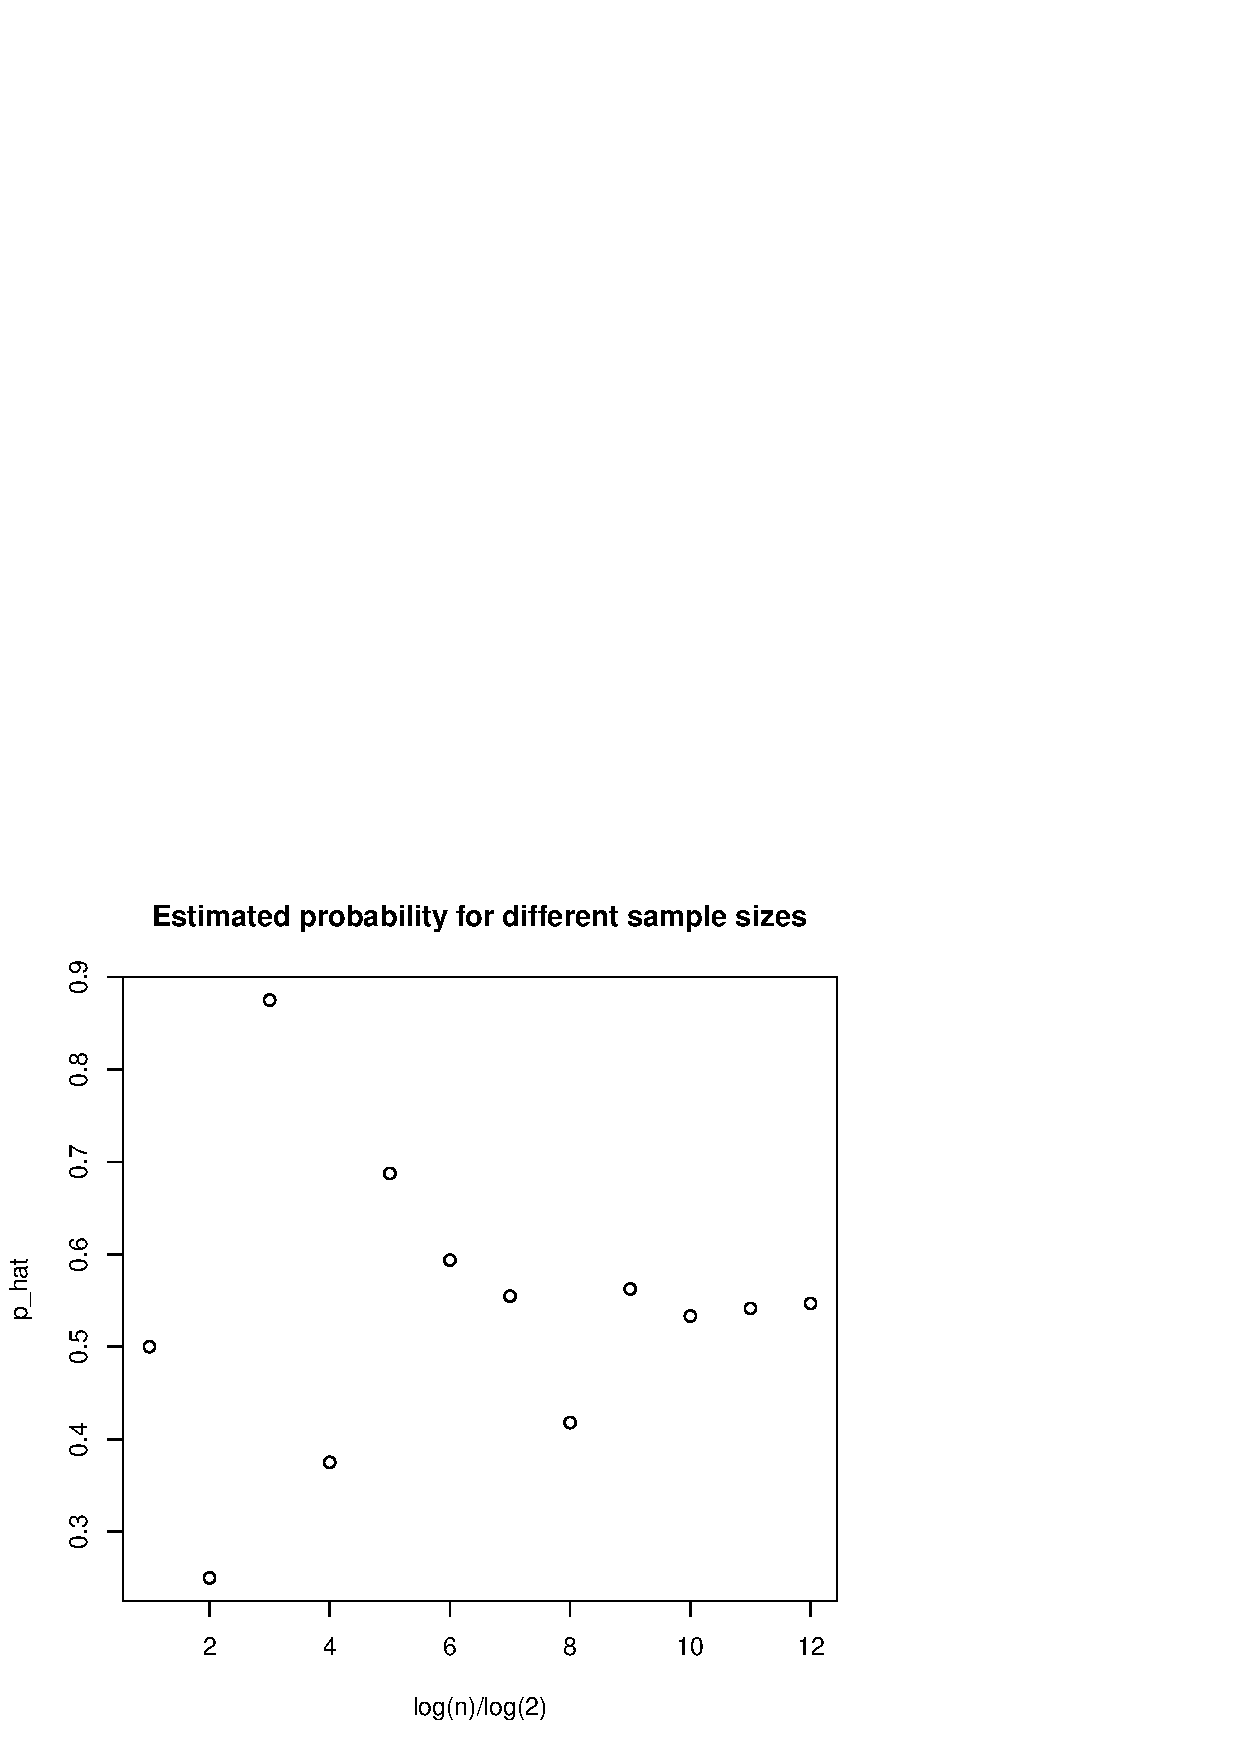
\includegraphics{spa1_tn248-squashgamesimulations}
\end{center}
\caption{Estimating $p(0.55,0.45)$ with a lot of games.}
\label{fig:squashgamesimulations}
\end{figure}

We see that it'll eventually converge to $.5$ as $k$ increases. On average, player 1 will win half of his points, whether it's his serve or not.

If we let $X_1,\ldots,X_n$ be an iid sample of Bernoulli(p) random variables, and let $\hat{p}=\bar{X}$ as an estimator of $p$, we have the following:

\begin{proposition}
	Var$(\hat{p})=p(1-p)/n.$
\end{proposition}

\begin{proof}
	Let \textbf{X}$=X_1 + \ldots + X_n$. We can use the identity
	\begin{align}
		\textbf{X}^2 &= \sum_{i=1}^n X_i^2 + 2 \sum_{i<j}X_iX_j\\
	\end{align}
	
	where $\sum_{i<j} X_iX_j = \sum_{i=1}^n \sum_{j=i+1}^n X_iX_j$. Because the expectation of $X_i^2 = 1^2p=p$, and the expectation of $X_iX_j=P(X_i=1,X_j=1)=p^2$, we get:
	
	\begin{align}
		E(\textbf{X}^2)&=E(\sum_{i=1}^n X_i^2 + E\left(2\sum_{i<j}X_iX_j)\right)\\
		&=\sum_{i=1}^n E(X_i^2)+2\sum_{i<j}E(X_iX_j)\\
		&=np+2 {n\choose 2 p^2}.
	\end{align}
	
	So, Var$(\textbf{X})=E(\textbf{X}^2)-(E(\textbf{X}^2))^2 = np(1-p)$, or Var $(\hat{p})=p(1-p)/n$.
\end{proof}

We now want to find some $n$ that will guarantee us that the standard deviation of $\hat{p}\leq 0.01$ for any value of $p$. So,

\begin{align}
	stdev \hat{p} &= \sqrt{p(1-p)/n}\\
	\sqrt{p(1-p)/n} &\leq .01\\
 	p(1-p)/n &\leq .0001\\
	p(1-p)/.0001 &\leq  n
\end{align}

	$p(1-p)$ takes a maximum value when $p=.5$, meaning that $n\geq 2500$. It's probably a good idea then, to simulate this many games for our $p(a,b)$ estimation table:
	
\begin{Schunk}
\begin{Sinput}
> resolution <- 250
> p.hat.values <- cbind(rep(seq(0.1, 0.9, by = 0.1), each = 9), 
+     rep(seq(0.1, 0.9, by = 0.1), 9))
> p.hat.table <- matrix(mapply(function(x, y) {
+     sum(mapply(play_game, rep(x, resolution), rep(y, resolution)))/resolution
+ }, p.hat.values[, 1], p.hat.values[, 2]), 9, 9, byrow = TRUE)
> p.hat.table
\end{Sinput}
\begin{Soutput}
       [,1]  [,2]  [,3]  [,4]  [,5]  [,6]  [,7]  [,8]  [,9]
 [1,] 0.000 0.000 0.000 0.000 0.004 0.000 0.012 0.076 0.496
 [2,] 0.000 0.000 0.000 0.004 0.016 0.028 0.160 0.544 0.940
 [3,] 0.000 0.004 0.008 0.024 0.124 0.220 0.444 0.856 1.000
 [4,] 0.004 0.000 0.032 0.128 0.252 0.544 0.792 0.964 1.000
 [5,] 0.012 0.044 0.152 0.308 0.564 0.812 0.912 0.988 1.000
 [6,] 0.076 0.188 0.320 0.584 0.700 0.936 0.976 1.000 1.000
 [7,] 0.132 0.320 0.596 0.744 0.888 0.976 0.996 1.000 1.000
 [8,] 0.336 0.624 0.764 0.888 0.976 0.996 1.000 1.000 1.000
 [9,] 0.664 0.844 0.924 0.972 0.996 1.000 1.000 1.000 1.000
\end{Soutput}
\end{Schunk}

The columns designate $b=.1, b=.2,\ldots, b=.9$, whilst the rows designate $a=.1, a=.2,\ldots, a=.9$. What's interesting to note is player 1's chances of winning are around $50$\%  along the anti-diagonal of this matrix, meaning any pair of $a,b$ values in the the lower anti-diagonal of the matrix guarantees a probability of over $50$\%. 

We would now like to calculate the average length of a game given various $a$ and $b$ values. We've rewritten \verb@play_game@ to simply count the number of points played. This new function is called \verb@play_game_length@, and can be found in the Appendix, or in this \texttt{.Rnw} file. 


Let's use \verb@play_game_length@ to create a table of expected lengths:

\begin{Schunk}
\begin{Sinput}
> length.table <- matrix(mapply(function(x, y) {
+     sum(mapply(play_game_length, rep(x, resolution), rep(y, resolution)))/resolution
+ }, p.hat.values[, 1], p.hat.values[, 2]), 9, 9, byrow = TRUE)
> length.table
\end{Sinput}
\begin{Soutput}
        [,1]   [,2]   [,3]   [,4]   [,5]   [,6]   [,7]   [,8]    [,9]
 [1,] 12.268 14.960 18.588 22.852 28.716 38.596 53.516 83.124 147.564
 [2,] 12.700 15.324 18.728 22.824 30.924 41.844 55.888 74.288  83.716
 [3,] 12.832 16.028 19.964 25.492 32.500 39.456 49.620 54.296  53.332
 [4,] 13.056 16.588 20.520 25.608 31.124 36.116 40.804 38.472  37.064
 [5,] 13.536 17.476 21.192 25.028 28.428 30.144 30.696 29.600  27.608
 [6,] 14.532 16.916 20.232 23.476 24.272 23.824 23.420 22.388  21.680
 [7,] 14.924 16.600 18.624 18.980 20.148 18.544 17.812 18.192  17.224
 [8,] 14.240 15.224 16.444 16.084 14.888 15.056 14.580 14.012  13.688
 [9,] 12.340 12.860 12.416 12.340 12.032 11.740 11.340 11.296  11.324
\end{Soutput}
\end{Schunk}

What's really interesting to me is that for very low $a$ values and very high $b$ values, we see some pretty long games. This makes sense though--if $a$ is the probability of scoring a point on a serve, and $b$ is the probability of winning your serve back, what's happening here is that player $1$ is failing to convert his serves into points, but is extremely good at getting his serve back from player $2$. In fact, if you set $a=0$ and $b=1$, you will get an never-ending game of squash. In all other corners though, we see fairly quick games--for example, for low $a$ and low $b$, we see player $2$ winning flat out after player 1 loses his serve. The quickest games occur when $a$ and $b$ are both high: in this case, we see player $1$ dominating both his serve points and his non-serve points.
\eans

% section a_game_of_squash (end)

\section{Population Dynamics (20)} % (fold)
\label{sec:population_dynamics}

We are now writing a simple model for density-independent population growth with spatial variation. Let $L$ denote the number of population patches along a line, $N_j(t)$ denote the population of patch $j$ at time $t$. $\lambda_j$ is the geometric growth rate in patch $j$. The equations that drive this model are as follows:

\begin{align}
	M_j(t) &=\lambda_j N_j(t) &\textrm{for all } j \\
	N_j(t+1) &= (1-2d)M_j(t)+dM_{j-1}(t)+dM_{j+1}(t) &\textrm{for } 2\leq j \leq L-1,
\end{align}

where $2d$ is the dispersal rate. Note there are special dispersal rules for the end patches. Let's try simulating this for $L=20$, $N_j(1)=5$ for all $j$, $t=1:50$, and $\lambda_j=.9$ in the left half, and $\lambda_j=1.2$ in the right half:

\begin{Schunk}
\begin{Sinput}
> L <- 20
> t.final <- 50
> initsize <- 5
> d <- 0.1
> lambda.one <- 0.9
> one.locations <- 1:10
> lambda.two <- 1.2
> two.locations <- 11:20
\end{Sinput}
\end{Schunk}


After we've written our functions to reflect the equations above, let's iterate the model from $t=1$ to $t=50$:

\begin{Schunk}
\begin{Sinput}
> for (i in 1:(t.final - 1)) {
+     population[i + 1, ] <- mapply(reflecting, rep(i, L), 1:L)
+ }
\end{Sinput}
\end{Schunk}

And then plot some sample patches:

\begin{Schunk}
\begin{Sinput}
> par(mfrow = c(3, 3))
> for (i in floor(seq(1, L, length = 9))) {
+     plot(1:t.final, log(population[, i]), xlab = "Time", ylab = "log(Population)", 
+         type = "l", main = paste("Patch ", i), ylim = c(0, log(max(population))))
+ }
\end{Sinput}
\end{Schunk}

\begin{figure}
\begin{center}
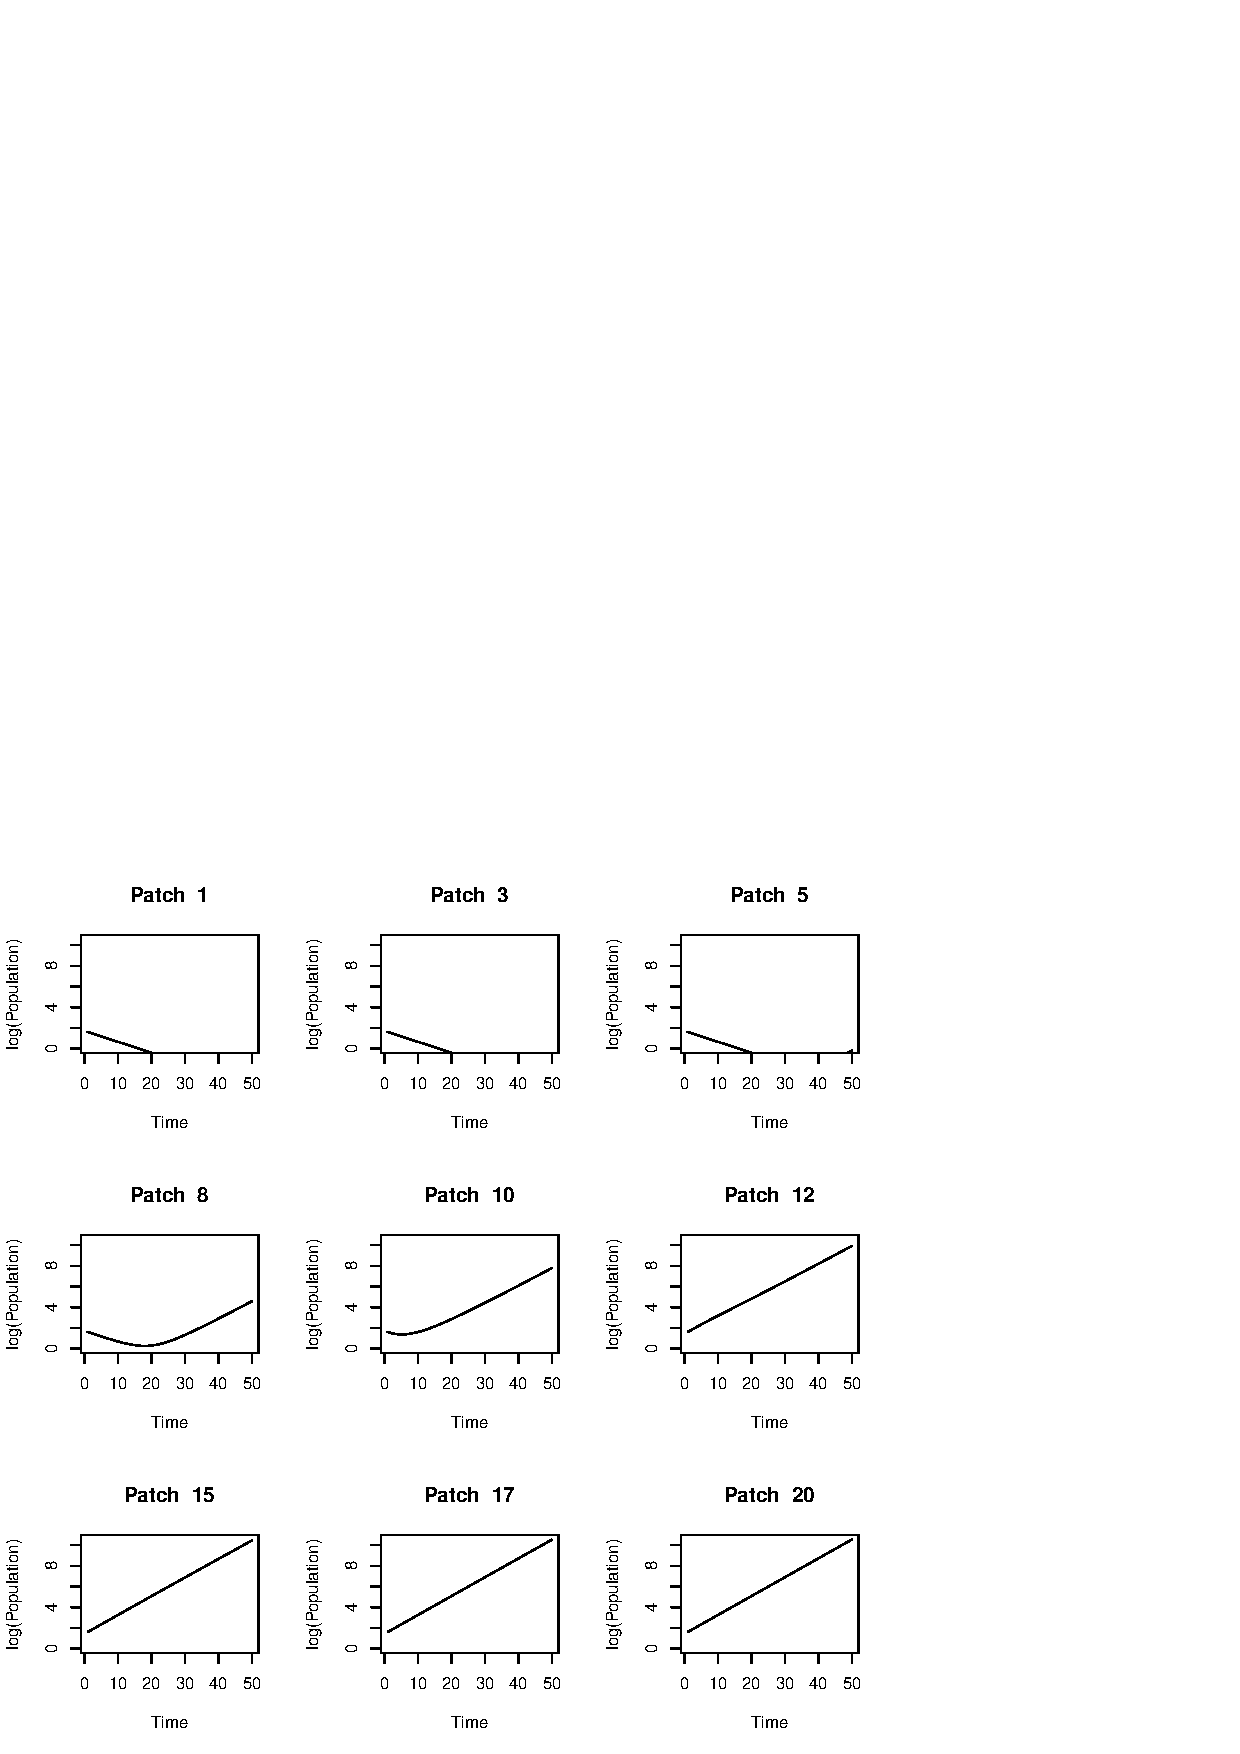
\includegraphics{spa1_tn248-popplot}
\end{center}
\caption{Log-plots of various patches with a good half/bad half setup.}
\label{fig:popplot}
\end{figure}

We see in Figure~\ref{fig:popplot} that the leftward most patch sees the sharpest population decline, and that the rightward most patch sees the sharpest population increase. Toward the center of the population line (Patch 10), we see a slight dip, followed by a sharp increase. It would seem that with two distinct lambdas on each side, we observe a spectrum of population trajectories, with the end patches being the extremes of population dearth and growth. What if we tried interspersing the good and bad patches?

\begin{Schunk}
\begin{Sinput}
> lambda.one <- 0.9
> one.locations <- c(1, 3, 5, 7, 9, 11, 13, 15, 17, 19)
> lambda.two <- 1.2
> two.locations <- c(2, 4, 6, 8, 10, 12, 14, 16, 18, 20)
\end{Sinput}
\end{Schunk}


\begin{figure}
\begin{center}
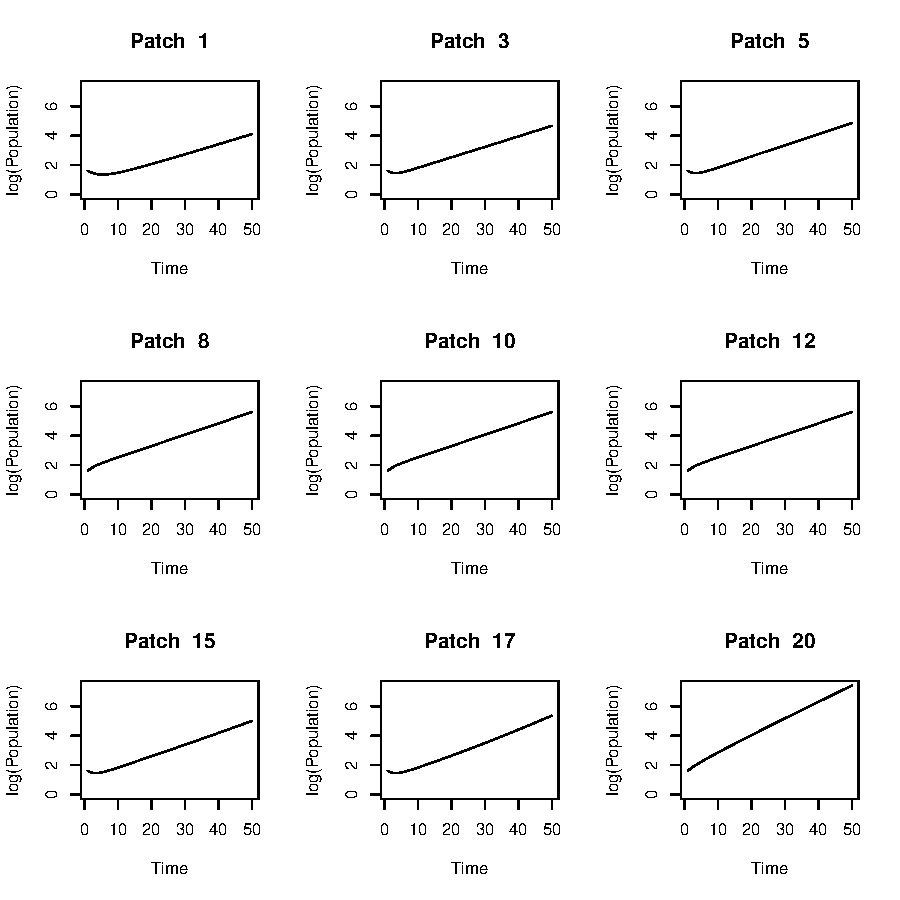
\includegraphics{spa1_tn248-popplot2}
\end{center}
\caption{Log-plots of various patches with alternating good/bad patches.}
\label{fig:popplot2}
\end{figure}

Figure~\ref{fig:popplot2} shows a pretty interesting result: on patches with the `bad lambda' rates, we see a slight dip in population to start, whereas with the patches with 'good lambda' rates see a slight hump in the population to start. Eventually, after a few iterations, both types of patches mellow out to the same, constant rate of growth. 

And what if we just made one good patch in the middle?

\begin{Schunk}
\begin{Sinput}
> lambda.one <- 0.9
> one.locations <- c(1:9, 11:20)
> lambda.two <- 1.4
> two.locations <- c(10)
\end{Sinput}
\end{Schunk}


\begin{figure}
\begin{center}
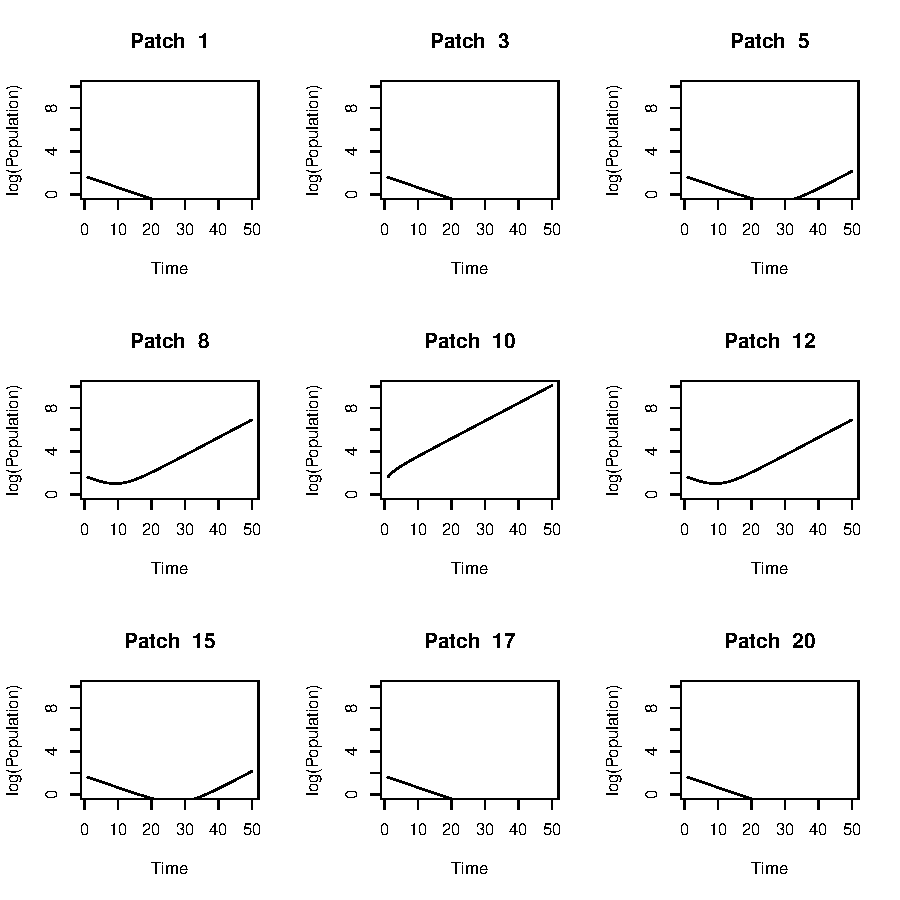
\includegraphics{spa1_tn248-popplot3}
\end{center}
\caption{Log-plots of various patches with one good patch in the middle.}
\label{fig:popplot3}
\end{figure}

Unsurprisingly, we observe symmetric trajectories as we move along the population line in Figure~\ref{fig:popplot3}. Patches 1-4 see a sharp population decrease to 0 by $t=20$; patch 5 is the first patch close enough to patch 10 to benefit from its dispersal, as we see a population uptick at $t=30$. The closer and closer we get to patch 10, the more pronounced the growth. Patch 10 will obviously be the fastest growing patch in the line, and as we move further and further to the right, we see a sort of symmetry to the patches left of patch 10, with patch 20 having an identical rate of decline as patch 1. 
% section population_dynamics (end)
\newpage
\section{Appendix: \texttt{spa1\_q1\_tn248.R}} % (fold)
\label{sec:appendix_1}

\begin{lstlisting}

# ##
# spa1_q1_tn248.R
# This script will compile scores, grades, and ranks for 
# an arbitrary number of students and their exam answers.
# It will also spot cheating by pairwise comparing students'
# answers and results.
# ##

# ##
# Created 14 Oct 2010
# Last updated 24 Oct 2010
# tn248@cam.ac.uk
# ##

num.students <- 12 # Adjustable
num.questions <- 30 #Adjustable
 
crib <- cbind(c(1:100),read.table("crib.dat"))
colnames(crib)<- c("qn","response")
rubric <- read.table("grade.txt",header=TRUE)

# initialize everything
student.index <-1:num.students
correct <-rep(NA,num.students)
rank<-rep(NA,num.students)

students <- lapply(1:num.students,function(x){read.table(paste(
	"student", toString(x),".dat",sep=""),header=TRUE)})

correct <- sapply(1:num.students,function(x){sum(students[[x]]$response ==
	 crib[students[[x]]$qn,]$response)})

number <- sapply(1:num.students,function(x){
	floor(100*correct[[x]]/num.questions)})

alpha.grades <- sapply(1:num.students,function(x){rubric$grade[
	which((rubric$min <= number[[x]]) == (number[[x]] <=
		 rubric$max), TRUE)]})

results <- data.frame(student=student.index,score=correct,
	grade=alpha.grades,rank=rank)

# assign ranks
results.sort<- results[order(results$score),]
results.sort$rank<-c(12:1)

# sort it back
results <- results.sort[order(results.sort$student),]
results
summary(results$score)

###
# cheater catcher function
###
# usage: cheaterkiller(i,j), where i and j are 
# the numbers of the suspected students
# 
# I had considered preloading all students before using 
# this function, but I think this is more memory efficient.

cheaterkiller <- function(i,j){ 
	
student.i <- read.table(paste("student", toString(i),".dat",sep=""),header=TRUE)
student.j <- read.table(paste("student", toString(j),".dat",sep=""),header=TRUE)

# which questions did they both attempt and how similar are the answers?
similarqs <- intersect(student.i$qn,student.j$qn)

#order by questions
student.i <- student.i[order(student.i$qn),]
student.j <- student.j[order(student.j$qn),]

#one-line to compare students' answers
similaras <- student.i$response[which(student.i$qn 
	%in% similarqs)] == student.j$response[which(
		student.j$qn %in% similarqs)]

return(sum(similaras))
	}
	
###
# Finding the cheater; only calculates lower diagonal of matrix
###

cheatermatrix <- matrix(rep(0,num.students^2),num.students,num.students)
x <- cbind(rep(1:num.students, each=num.students),rep(1:num.students, num.students))
x <- x[x[,1] <= x[,2], ]
cheatermatrix[lower.tri(cheatermatrix,diag=TRUE)]<-mapply(cheaterkiller,x[,1],x[,2])
cheatermatrix
\end{lstlisting}

% section appendix_ (end)

\newpage

\section{Appendix: \texttt{spa1\_q2\_tn248.R}} % (fold)
\label{sec:appendix_texttt_spa1_q2_tn248_r}

\begin{lstlisting}
# ##
# spa1_q2_tn248.R
# This script will simulate a game of squash.
# It will then simulate many games of squash, and plot
# some p.hat estimations.
# ##

# ##
# Created 27 Oct 2010
# Last updated 28 Oct 2010
# tn248@cam.ac.uk
# ##

library(spuRs)

# The following two functions were taken from the spuRs
# package, a companion to Scientific Programming Using R 
# by Jones, Maillardet, and Robinson.

status.test <- function(s.ftn){
	x.vec <- (-1):11
	y.vec <- (-1):11
	plot(x.vec, y.vec, type = "n", xlab="x",ylab="y")
	for(x in x.vec){
		for(y in y.vec){
			s <- s.ftn(x,y)
			if (s == "impossible") text(x,y,"X",col="red")
			else if (s == "unfinished") text(x,y, "?", col="blue")
			else if (s == "player 1 win") text(x,y,"1", col="green")
			else if (s == "player 2 win") text(x,y,"2", col="green")
			}
		}
	return(invisible(NULL))
}

play_game<- function(a,b){
	state <- c(0, 0, 1) # player 1 serves first
	while (status(state[1],state[2]) == "unfinished"){
		#show(state)
		state <- play_point(state, a, b)
		}
	if (status(state[1],state[2]) == "player 1 win"){
		return(TRUE)
	} else{
		return(FALSE)
	}
}

# The rest is mine.

status <- function(x,y){
	if (x < 0 | y < 0 | (x > 9 & x-y > 2) | (y > 9 & y-x >2)){
		return("impossible")}
	else if((x == 9 & x-y >= 2) | (x > 9 & x-y == 2)){
		return("player 1 win")}
	else if((y == 9 & y-x >= 2) | (y > 9 & y-x == 2)){
		return("player 2 win")}
	else{return("unfinished")}
	}

play_point <- function(state,a,b){
	# for my reference:
	# state = (x,y,z)
	# x is player 1's score
	# y is player 2's score
	# z indicates whose serve
	# a is probability 1 wins a point when 1 serves
	# b is probability 1 wins a point when 2 serves
	if (state[3]==1){
		odds <- a}
	else{odds <-b}
		
	# the game!
	point <- rbinom(1,1,odds)
	
	if (point == 1){
		if (state[3]==1) {state[1] <- state[1] + 1}
		else if (state[3]==2) {state[3] <- 1}
		}
	else if (point == 0){
		if (state[3]==1) {state[3] <- 2}
		else if (state[3]==2) {state[2] <- state[2] +1}
		}
	
	return(state)
	}

# The seed is my birthday, in American date form. 
# Set once and only once.
seed <- 110685
set.seed(seed)

# Estimating probability for different sample sizes
sample.size <- 12
probabilities <- rep(NA,sample.size)

# this will take a while
probabilities <- sapply(1:sample.size,function(x){sum(mapply(
		play_game,rep(.55,2^x),rep(.45,2^x)))/2^x})

plot(1:sample.size, probabilities,main="Estimated probability 
	for different sample sizes", xlab="log(n)/log(2)", ylab="p_hat")

# Table of estimated p(a,b) values
resolution <- 250
p.hat.values <- cbind(rep(seq(.1,.9,by=.1),each=9),rep(seq(.1,.9,by=.1),9))

# This one-liner will create a table of p.hats by simulating 
# games for each pair in p.hat.values. Might take a while depending on
# the resolution.
p.hat.table <- matrix(mapply(function(x,y){sum(mapply(play_game,rep(x,resolution),
		rep(y,resolution)))/resolution},p.hat.values[,1],p.hat.values[,2]),
			9,9,byrow=TRUE)

play_game_length <- function(a,b){
	state <- c(0, 0, 1) # player 1 serves first
	count <- 0
	while (status(state[1],state[2]) == "unfinished"){
		#show(state)
		state <- play_point(state, a, b)
		count <- count + 1
		}
	if (status(state[1],state[2]) == "player 1 win"){
		return(count)
	} else{
		return(count)
	}
}

length.table <- matrix(mapply(function(x,y){sum(mapply(play_game_length,rep(x,resolution),
		rep(y,resolution)))/resolution},p.hat.values[,1],p.hat.values[,2]),9,9,
			byrow=TRUE)
length.table
\end{lstlisting}

% section appendix_texttt_spa1_q2_tn248_r (end)

\newpage

\section{Appendix: \texttt{spa1\_q3\_tn248.R}} % (fold)
\label{sec:appendix_texttt_spa1_q3_tn248_r}

\begin{lstlisting}
# ##
# spa1_q1_tn248.R
# This script will simulate a simple model 
# for density-independent population
# growth with spatial variation, as per 
# Exercise 10 in "An introduction to R 
# for dynamic models in biology". 
# ##

# ##
# Created 18 Oct 2010
# Last updated 26 Oct 2010
# tn248@cam.ac.uk
# ##

# parameters, adjustable
L <- 20 # how many patches?
t.final <- 50 # how many iterations?
initsize <- 5 # what's our initial population in each patch?
d <- 0.1 # what's the dispersal rate? (important: it's 2*d)

# what and where are the growth rates?
lambda.one <- 1.2
one.locations <- 1:10 #c(1,3,5,7,9,11,13,15,17,19) # for maximum flexibility

lambda.two <- .9
two.locations <- 11:20 #c(2,4,6,8,10,12,14,16,18,20)

# initialize everything up
population = matrix(rep(0,L*t.final), t.final,L)
population[1,] = rep(initsize,L)

onegrowth <- function(t,j){
	geogrowth <- lambda.one * population[t,j]
return(geogrowth)
}

twogrowth <- function(t,j){
	geogrowth <- lambda.two * population[t,j]
return(geogrowth)
}

# This function will take N_j(t) and produce N_j(t+1)
reflecting <- function(t,j){#not entirely happy with this

if(j %in% one.locations)
	{
		type = "one"
		if (j==1){type= "leftendone"}
		if (j==L){type= "rightendone"}	
	}
if(j %in% two.locations)
	{
		type = "two"
		if (j==1){type= "leftendtwo"}
		if (j==L){type= "rightendtwo"}
	}

newpop <- switch(type, 
	leftendone = (1-d)*onegrowth(t,j) + d*onegrowth(t,j+1),
	leftendtwo = (1-d)*twogrowth(t,j) + d*twogrowth(t,j+1),
	one = (1 - 2*d)*onegrowth(t,j) + d*onegrowth(t,j-1) + 
					d*onegrowth(t,j+1),
	two = (1 - 2*d)*twogrowth(t,j) + d*twogrowth(t,j-1) + 	
				d*twogrowth(t,j+1),
	rightendone = (1-d)*onegrowth(t,j) + d*onegrowth(t,j-1),
	rightendtwo = (1-d)*twogrowth(t,j) + d*twogrowth(t,j-1),
			)
return(newpop)
	}

# This will produce populations for t+1
for(i in 1:(t.final-1)){
population[i+1,]<- mapply(reflecting,rep(i,L),1:L)
}

par(mfrow=c(3,3))
for (i in floor(seq(1,L, length=9))){
plot(1:t.final,log(population[,i]), xlab="Time", ylab="log(Population)",
type="l", main=paste("Patch ", i),ylim=c(0,log(max(population))))
}
\end{lstlisting}

% section appendix_texttt_spa1_q3_tn248_r (end)
\end{document}
